
\begin{figure}[H]
    \begin{minipage}[b]{0.3\linewidth}
        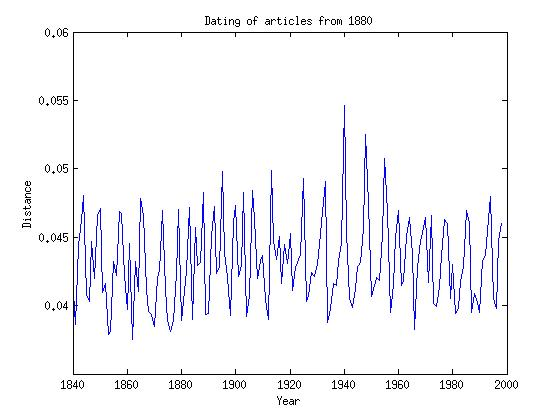
\includegraphics[scale=0.25]{Pictures/date_articles/cos/dating1880.jpg}
        \caption{Dating articles from 1880 with the cosine distance. Prediction is 1862.}
    \end{minipage}\hfill
    \begin{minipage}[b]{0.3\linewidth}
        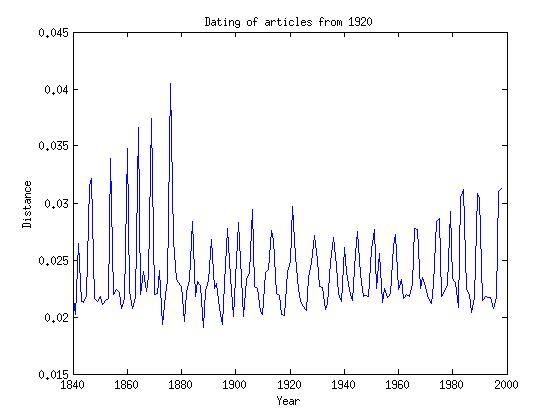
\includegraphics[scale=0.25]{Pictures/date_articles/cos/dating1920.jpg}
        \caption{Dating articles from 1920 with the cosine distance. Prediction is 1889.}
    \end{minipage}\hfill
    \begin{minipage}[b]{0.3\linewidth}
	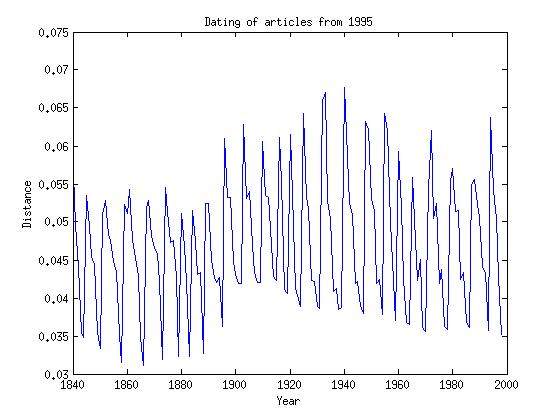
\includegraphics[scale=0.25]{Pictures/date_articles/cos/dating1995_corrected.jpg}
        \caption{Dating articles from 1995 with the cosine distance. Prediction is 1866}
        \label{date_cos}
    \end{minipage}
\end{figure}
The cosine distance seems to have the same behaviour as the basic and \emph{Chi-Square} distances for dating. Its predictions are also not accurate.